\minitoc
% \startcontents[chapters]
% \printcontents[chapters]{}{1}{}

\section{Introduction}
\label{sec:buildability:intro}

% Rodr\'iguez-P\'erez et al. have found that bugs have two types of origins~\cite{rodriguez2018if}.
% There are intrinsic bugs, introduced by the lines of code that were modified to fix it, and extrinsic bugs, introduced by changes not registered in the source code management systems (e.g., by an external dependency).
% Identifying what type of bug we have is currently a labor-intensive task that has to be done manually.
% To a major extent it has to cope with the question if the lines that the SZZ algorithm~\cite{sliwerski2005changes} identifies as the Bug-Introducing Change (BIC) were correct or not. 
% In the case they were not correct, we would have an intrinsic bug; otherwise, we face an extrinsic bug.

% We therefore aimed to automate the process with following idea: running a regression test for the BIC candidate.
% This means running tests on past versions of the software.
% The snapshot (commit) where the test fails would be the candidate for being the BIC~\cite{kim2006automatic}.
% To do this, it is however necessary to first build, and then run the regression test on the previous snapshots of the project.
% When doing this, we found that many of the snapshots were not compilable. %\patxi{Explicar claramente que los commits en rojo se produjeron por algún motivo. ¿Estamos seguros que estaban en rojo? Igual no tenía CI, y no se verificó. Habria que explicar que esos builds que no compilan no se pueden reproducir. Comentar ejemplos concretos.Referenciar el estado del arte para indicar que esto se sigue produciendo.}
% We discovered that when the build failed, in some cases the failure was the original outcome of the build (i.e., there was a bug in the project or some changes broke the build), but in other cases, the problem was that we were not able to reproduce the environment conditions necessary for the build to succeed. \grex{Reescribir esta \'ultima frase que es un poco cr\'iptica.}

% That way, our original aim (running regression tests on past versions of the software) required first to solve the problem of how to first build these past versions of the software. 
% Inspecting the literature, we have found that we are not the only ones interested in such a topic.

The problems for building the current snapshot from source code has been discussed in detail in the research literature (see Section~\ref{sec:buildability:related}), but the problems for \textbf{building past snapshots} have received less attention. 

Compilability of past snapshots of the source code of a software product has been shown to be of interest both for researchers and practitioners~\cite{nikitin2017chainiac,RepBlds:2017:Online}. 
Some examples of its uses are:
\begin{inparaenum}[\bf(1)]
	\item {\bf to search and find bugs} developers often run previous snapshots of the system in order to locate bugs and understand how they originated~\cite{Zimmermann:2006:MVA:1137983.1138001};
	\item {\bf due to security reasons} users usually trust available binaries of a library, but a backdoor could have been introduced~\cite{deCarnedeCarnavalet:2014:CIV:2664243.2664288}, so rebuilding it from the original source allows to compare the binaries and verify that it was not modified; 
	\item {\bf to backport bug fixes} it is necessary to build an old version to apply a patch to that specific version of the software~\cite{tian2017mining}); and
	\item {\bf to reproduce the past state of a system}, for research purposes, it is useful to obtain a functional executable to verify the correct performance of the system~\cite{manacero2011using}, or to use the project history to predict future bugs~\cite{Zimmermann2008}).
\end{inparaenum}

To our knowledge, the most complete study on the compilability of all past snapshots is presented in~\cite{tufano2017there} (from now on ``the original paper'' or ``the original study''). It analyzes all past snapshots for 100 Java projects of one organization (the Apache Software Foundation, ASF), determining how many of them could be built, and the main causes of failure in building. Its main conclusions were: only 38\% of snapshots could be successfully built, almost all projects contained snapshots that could not be built (96\%), and the main cause of failure when building a snapshot was dependency resolution. In this chapter, we decided to revisit and extend this paper, with two main aims:

\textbf{(1)} To validate the results of the original study, by trying to build {\bf in 2020} the same snapshots it considered {\bf in 2014}, answering the original two research questions (although slightly rephrased):

\textbf{RQ\textsubscript{1.1a}}: ``How many snapshots from the change history are compilable?''

\textbf{RQ\textsubscript{1.1b}}: ``Which types of errors prevent snapshots from being built?''

We reproduced the conditions and methodology of the original study as much as possible, studying compilability of the same snapshots with the Maven tool, as they did. 
In addition, we also wanted to learn if compilability had degraded. We suspected that it could be the case because one of the main reasons for failed builds in the original study was availability of dependencies, which is known to degrade over time~\cite{bavota2015apache}. So we added the following research question:

\textbf{RQ\textsubscript{1.1c}}: ``Has compilability degraded since the original study?''

While answering the previous RQs, we stumbled upon some problems that lead us to an additional one:

\textbf{RQ\textsubscript{1.1d}}: ``Are the data in the reproduction package of the original study enough for a replication?''

\textbf{(2)} To explore the generalizability of the results, by conducting another study with the same methodology but on a  set of Java projects with a more diverse background:

\textbf{RQ\textsubscript{1.2a}}: ``How many snapshots from the change history are compilable?''

\textbf{RQ\textsubscript{1.2b}}: ``Which types of errors prevent snapshots from being built?''

\textbf{RQ\textsubscript{1.2c}}: ``Are there differences in compilability depending on the building tool?''

With the first two questions, we check the extensibility of the results of the original paper to other Java projects. 
The last question is aimed to find out if some building tools perform better in terms of compilability than others, for example because of the amount of information they require about the construction process and the construction context.

In the rest of this chapter, we refer to the study that addresses RQ\textsubscript{1.1[a-d]} as \emph{replication study}, and \emph{reproduction study} to the one answering RQ\textsubscript{1.2[a-c]}. 
This terminology is based on~\cite{juristo2010replication} and~\cite{cartwright1991replicability}, which distinguish between \textbf{replication} (performing the same experiment again) and \textbf{reproduction} (performing the same experiment but with other input/data). Very recently, this terminology has been reviewed,\footnote{https://www.acm.org/publications/policies/artifact-review-and-badging-current} however in this paper we use the traditional definitions for replication and reproduction studies.

Our replication study analyzes 79 projects from the set of 100 in the original study, and our reproduction study will be performed on a dataset of 80 FOSS (free, open source software) Java projects. In addition, for the reproduction we will extend the build systems with Ant (very popular in the old days of long-running projects) and Gradle (a newer build tool) -- the original study only considered Maven. In both studies we used our own software for checking compilability and analyzing the resulting logs (see Section~\ref{sec:buildability:repro}).




% jgb: TODO. Likely we should move the following text to the conclusions.

%Furthermore, the ASF is a decentralized open-source community of developers, whose projects have been extensively researched~\cite{roberts2006understanding, iqbal2014understanding, kabinna2016logging, bavota2015apache, bavota2013evolution}.
%We cannot be confident that the conclusions obtained by Tufano et al. are also applicable to other open-source projects outside the Apache Foundation, given the strict rules that apply to projects pertaining the ASF\footnote{https://www.apache.org/foundation/how-it-works.html}. 



% In this paper, we argue that compilability should not be limited to the current (i.e., latest) version of a software, but to all its history (or at least part of it) -- we refer to this ability as {\bf historic compilability}, and in particular to {\bf complete historic compilability} when \emph{all past versions of a software project can be built}.

% We have studied the compilability of the history of several projects checking if their snapshots are compilable or not, and accounting the different errors and their duration in time.
% We have focused on five well-known open source Java projects, which are taken from the Defects4J repository~\cite{Just:2014:DDE:2610384.2628055}, commonly used in Software Engineering research. Our expectation is that most of the snapshots of a project are compilable, as they usually have continuous integration (CI) environments that compile and test the code to find issues before submitting changes to the repository. Even when there is no CI environment, it is expected that developers will compile and test their changes before submitting them. 


%\jgb{Review the next para, to ensure it matches reality}

The rest of the chapter is structured as follows:
% Section~\ref{sec:buildability:related} discusses previous research. 
Section~\ref{sec:buildability:definitions} defines the main concepts.
Section~\ref{sec:buildability:metodology} presents the methodology used in the studies. 
The results of applying the methodology are reported in Sections~\ref{sec:buildability:results-repli} (replication) and~\ref{sec:buildability:results-repro} (reproduction).
Section~\ref{sec:buildability:discussion} discusses the results, and explores threats to their validity.
Finally, Section~\ref{sec:buildability:conclusions} draws conclusions and presents further research.


\section{Previous Research}
\label{sec:buildability:related}
The build process and the errors preventing correct builds, have been an active area of research during the last years.
One of the most influential empirical studies in this area was authored by Seo et al., who examined 26.6 million builds from Google's centralized build systems, analyzing compilation errors in failed builds. As a result, an error taxonomy was provided based on log patterns~\cite{Seo:2014:PBE:2568225.2568255}.
Sulír and Porubän examined the builds of more than 7,000 Java projects, but only for their last commit~\cite{Sulir:2016:QSJ:3001878.3001882}. 
Other investigations have also focused on errors related to build failures. 
Rausch et al. address specifically the reasons why builds fail in the context of CI environments~\cite{Rausch:2017:EAB:3104188.3104231}.
Travis logs from 14 open-source projects were analyzed, finding that a significant fraction of errors corresponded to tests that failed because of a failure in a previous build.
The study analyzed the build logs from the point of view of continuous integration systems (snapshot build and test execution), but it did not include a reproduction of the builds.
Some authors have emphasized the importance of historic compilability to propose repair tools for failed builds.
Using a taxonomy for the root causes of build failures found in 86 out of the 200 most popular Java projects in GitHub, it was demonstrated that 52 of these failures could be resolved in an automated manner~\cite{hassan2017automatic}.
And the \texttt{HireBuild} tool was able to fix 11 out of 24 reproducible build failures using fix patterns automatically generated from existing build script fixes and recommending fix patterns based on build log similarity~\cite{HireBuild}.
None of the previous studies considered historic compilability, which is the subject of our study. They were in general based on the analysis of logs: in comparison, our studies perform our own building processes, starting from scratch with the source code available in the analyzed snapshots.

A related area to compilability is build reproducibility: \emph{``the ability to generate byte-to-byte identical binaries from the source code of a project version, no matter who builds the binary, when or in which machine''}~\cite{RepBlds:2017:Online}. 
Reproducible builds create a verifiable path from human readable source code to the binary code used by computers, and are gaining relevance~\cite{cito2017empirical,maudoux2018correct,deCarnedeCarnavalet:2014:CIV:2664243.2664288,perry2014reproducible}. 
Software compilations, such as Debian and other Linux-based distributions, have a strong interest in the build reproducibility~\cite{RepBlds:2017:Online,RepBlds:2017:Online}. Obtaining reproducible builds in Debian has been addressed in~\cite{Glukhova:Thesis:2017} and~\cite{Ren:2018:ALU:3180155.3180224}, which present tools to ensure reproducibility, and a framework for detecting and fixing packages with problems. 
However, they focus on the latest version, not dealing with past reproducibility.

The reproducibility of builds is also interesting from a security point of view.
Some works focus on bringing security into the software development life cycle, considering build reproducibility as one of the main issues to be taken into account. Proposals have been presented to use reproducible builds in the context of security-critical open source software~\cite{deCarnedeCarnavalet:2014:CIV:2664243.2664288}, decentralized software-update frameworks including build verifiers~\cite{nikitin2017chainiac}, systems to ensure binary transparency~\cite{hassan2017automatic}, or enhancing trust in software through reproducible builds~\cite{Skrimstad:Thesis:2018}.
Even when our work is relevant to obtain reproducible builds of past versions of the software, we have not dealt with the details needed to ensure it.

Compilability of past versions of a program has been used instrumentally in research or industrial activities.
This is the case for bug location~\cite{Sliwerski:2005:CIF:1083142.1083147,Asaduzzaman:2012:BIC:2664446.2664463,Murgia:2010:MLA:1852786.1852794,Zimmermann:2006:MVA:1137983.1138001,Zimmermann2008}.
When locating bugs, techniques like GitBisect~\footnote{\url{https://git-scm.com/docs/git-bisect}} may be used to traverse the project history of commits back to the past, to find the change that introduced a bug~\cite{spinellis2012git,meneely2013patch}. 
In these cases, the utility of the technique is limited to tools performing static analysis, except when automatic compilability of past snapshots can be ensured -- then, the debugged system can be also analyzed dynamically.
Some authors have proposed metrics to evaluate the stability of project builds over time~\cite{6405296}.
Others have addressed the problem in an indirect way, for example when trying to run mutant tests in previous versions of several software projects~\cite{Just:2014:MVS:2635868.2635929} provided by Defects4J~\cite{Just:2014:DDE:2610384.2628055}. However, none of those studies systematically addresses the analysis of the compilability of past versions of real systems.

Build breakage repair techniques have been also proposed. Macho et al. derived three automatic repair techniques from 37 broken Maven builds~\cite{macho2018automatically}. 
Using these techniques, they were able to automatically fix 45 of an additional 84 broken builds. 
Other authors used a different strategy to achieve higher compilability. Behnamghader et al. focus solely on a module within the software (the one that changes)~\cite{behnamghader2018scalable}. They achieved high compilability for the three different datasets considered (Apache, Google and Netflix), above 94\% in all cases. Surprisingly, another work by He et al. has found that the presence of broken builds did not result in an increase of commit frequency (thus working on solving the breakage)~\cite{he2020characteristics}. The authors also reported a correlation between tags like \textit{feature add} or \textit{refactoring} linked to a broken build, after studying 68 Java repositories.

The most complete study on the compilability of all past snapshots is presented by Tufano et al.~\cite{tufano2017there}.
This work will be the direct precedent of the studies we present on Chapter~\ref{chapter:buildability}. 
Thus, its methodology and results will be discussed in detail later in this chapter.

A study of past snapshots to detect bug-introducing commits is tackled by Querel et.al~\cite{querel:2021:warning}. 
The authors partially replicate the work by Tufano et al., by trying to improve the compilability of eight of the Maven-based projects. 
They do so by solving the \textit{missing dependency} problem, selecting a dependency close to the commit date. 
Through this technique a compilability of 78.4\% is reported -- doubling in compilability compared to prior work. For those commits whose build fail, they run the \texttt{findbugs} tool~\cite{ayewah2007using} in an attempt to understand if the failure could be caused by a bug. 
Their results were negative, although developers found the reports offered by \texttt{findbugs} useful.


\section{Definitions}
\label{sec:buildability:definitions}
We derive the terminology used in this chapter from Sul\'ir and Porubän~\cite{Sulir:2016:QSJ:3001878.3001882}. According to it, the build process of projects programmed with compilable languages consists of following steps:
\begin{inparaenum}[\bf(1)]
    \item \textbf{read} the project build (configuration) file,
    \item \textbf{download} third party components defined in the build file,
    \item \textbf{execute} the compiler to generate  binary files from source code, and
    \item \textbf{package} the program in a suitable format for deployment.
\end{inparaenum}

A specific project version is {\bf compilable}\footnote{Although Sul\'ir and Porubän use the term \textit{buildable}, for consistency we have used the term \textit{compilable} instead, as in the study by Tufano et al., which we would like to replicate and reproduce.} if these steps can be executed to generate a valid binary, with a success build status. Based on this background, we define:

\begin{itemize}
\item \textbf{Snapshot}: a version of the source code of a project, represented by a commit of its git repository. It will be identified by the unique hash of the commit.
\item \textbf{Snapshot with build configuration}: a snapshot with configuration files for a build system.
\item \textbf{Successful build}: a snapshot that was compilable (\emph{we could build it})
\item \textbf{Failed build}: a snapshot that could not be built.
\item \textbf{Error for a build}: a failing build (and its cause).
\end{itemize}


\section{Methodology}
\label{sec:buildability:metodology}
For both our replication and reproduction studies we use a similar workflow, sketched in Figure~\ref{fig:methodology}. We work with git repositories, which means that we can clone the whole repository locally, and that each code snapshot corresponds to a commit in the git history of the repository. We locate repositories to analyze, clone them, and try to find out all the commits of interest. If we cannot clone a repository, or we do not find all the commits of interest in it, we discard it. Then, for each remaining repository, we get its commits of interest, and for each of these commits we investigate if it uses a building system. If so, we try to build it.

\begin{figure}[ht!]
\centering    
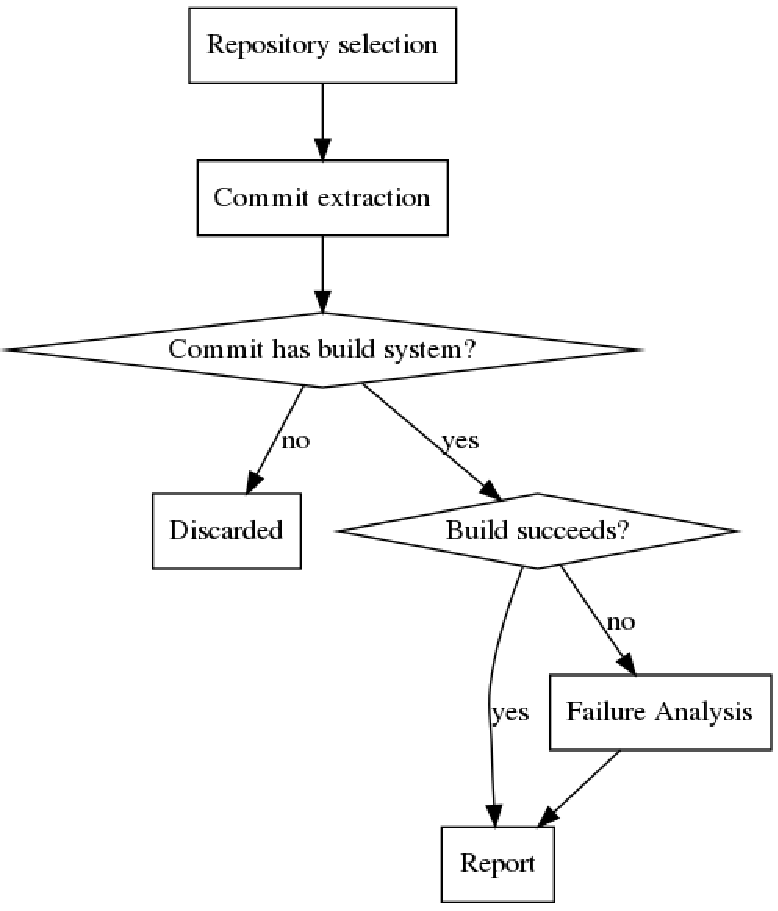
\includegraphics[height=0.8\textwidth]{pages/01-Buildability/images/Methodology.pdf}
\caption{Basic workflow for both studies.}
\label{fig:methodology}
\end{figure}


% Reduce separation between cells in next table
\renewcommand{\tabcolsep}{3pt}

\begin{table}[h]
\caption{Studies (main quantities)}
\label{table:statistics}
\begin{center}
\begin{tabular*}{\textwidth}{@{\extracolsep{\fill}}lrrrr}
\toprule
\textbf{Studies:}        & \textbf{Original} & \textbf{Original} & \textbf{Replic.} & \textbf{Reprod.} \\
                         & \textbf{Pristine} & \textbf{Reduced} \\
\midrule
Repositories             & 100               & 79                & 79               & 80      \\
Commits                  & 174,505           & 139,389           & 139,389          & 300,873 \\
Commits (build conf.)    & 132,484           & 101,811           & 101,811          & 281,487 \\
Commits (build success)  & 31,696            &  22,737           & 14,664           & 98,488  \\
\bottomrule
\end{tabular*}
%\caption*{
%  }
\end{center}

\begin{center}
\begin{tabular*}{\textwidth}{@{\extracolsep{\fill}}lrrrrrrr}
\toprule 
\textbf{Commits/project}  & \bf{min} & \bf{25\%} & \bf{50\%} & \bf{mean}  & \bf{75\%} & \bf{max}  & \bf{std} \\

\midrule
\bf{Replication}   &       25 &          234 &         726 &    1,764 &       1,898 &    14,818 & 2,694 \\
\bf{Reproduction}  &    1,132 &        1,974 &       2,980 &    3,760 &       4,847 &    10,000 & 2,404 \\


% Dejo esto aqui por si utilizamos estas cabeceras
% \bf{mean}  & 1,764.41  & 3,111.13 \\
% \bf{std}   & 2,694.93  & 1,825.44 \\
% \bf{min}   & 25       & 1,147    \\
% \bf{25\%}  & 234      & 1,791    \\
% \bf{50\%}  & 726      & 2,401    \\
% \bf{75\%}  & 1,898     & 3,693    \\
% \bf{max}   & 14,818    & 7,847    \\


\bottomrule
\end{tabular*}
\end{center}

\end{table}

% Restore original separation between cells
\renewcommand{\tabcolsep}{6pt}

There are some differences between the two studies, mainly on how we find repositories, which ones are our commits of interest in them, how we find those commits, and which build systems we consider (see details below). Table~\ref{table:statistics} shows some quantification (projects and commits) for the original study, with all its projects (\textit{Original Pristine}), for the reduced version of it, with the 79 repositories in which we could find all the commits (\textit{Original Reduced}), and for our replication (considering Maven builds only) and reproduction studies. The distribution of commits per project for the replication and reproduction studies is given as well.

% % Reduce separation between cells in next table
% \renewcommand{\tabcolsep}{3pt}

% \begin{table}[h]
% \caption{Basic statistics of projects}
% \label{table:statistics}
% \begin{center}
% \begin{tabular}{rrrrrrrr}
% \toprule 
% \bf{Study}    & \bf{min} & \bf{25\%} & \bf{50\%} & \bf{mean}  & \bf{75\%} & \bf{max}  & \bf{std} \\

% \midrule
% \bf{Replication}   &       25 &          234 &         726 &    1,764.41 &       1,898 &    14,818 & 2,694.93 \\
% \bf{Reproduction}  &    1,147 &        1,791 &       2,401 &    3,111.13 &       3,693 &     7,847 & 1,825.44 \\


% % Dejo esto aqui por si utilizamos estas cabeceras
% % \bf{mean}  & 1,764.41  & 3,111.13 \\
% % \bf{std}   & 2,694.93  & 1,825.44 \\
% % \bf{min}   & 25       & 1,147    \\
% % \bf{25\%}  & 234      & 1,791    \\
% % \bf{50\%}  & 726      & 2,401    \\
% % \bf{75\%}  & 1,898     & 3,693    \\
% % \bf{max}   & 14,818    & 7,847    \\


% \bottomrule
% \end{tabular}
% \end{center}
% \end{table}

% % Restore original separation between cells
% \renewcommand{\tabcolsep}{6pt}

\subsection{Replication Study}

For the replication study we followed the methodology of the original study as much as possible. Its authors considered 100 git repositories corresponding to Java FOSS projects from the ASF, all of them using a Maven-based build infrastructure. They retrieved in September 2014 all commits in their master branches, claiming to have analyzed a total of 219,395 commits. Then, they attempted to build all of them locally using Maven. The original paper comes with an accompanying reproduction package listing in detail which commits they considered for each repository. When reviewing that list, we found that the total number of commits referenced is 174,505. This is the reason why this is the number we include in the tables for the original study (see details in Section~\ref{sec:buildability:results-repli}).

\subsubsection{Subject Recovery}

Our first step was to retrieve the git repositories to analyze. We wanted to clone all the repositories, to be able of checking out each specific commit, and analyze its compilability. We were interested in doing a replication as close as possible, so we decided to use only the repositories for which we could find all the commits of the original study. This way, we ensured that results would be comparable, and not influenced by a potentially biased sample of missing commits.

We started by using the list of git repositories from the original study to clone and check all of them. We noticed that some were not available or did not have all the commits considered in the original study. From a total of 100 repositories in the list, 6 were no longer available. Before discarding them, we tried to find them both in the ASF git repositories, and in the GitHub repositories that the foundation maintains as replicas of the original ASF-hosted ones. In addition, of those that we could clone, 19 did not have all of the commits considered in the original study (8 had none of them, 11 had only some of them). This resulted in a total of 75 repositories with the complete set of commits considered in the original study. We followed this procedure during February 2020.

To improve the number of repositories with all commits from the original study,  we turned on to Software Heritage (SH), an initiative to collect, preserve and share all public source code in a universal software archive~\cite{di2017software,di2018software}. SH tries to archive all commits, even if they are later removed from the original repositories. Therefore, it was an option for finding the missing commits. Although its API is still evolving, during March 2020 we could use it to retrieve some of the repositories with missing commits, or which we could not find\footnote{In later conversations with representatives of Software Heritage, we learned that the part of the API for retrieving full repositories had been removed because it failed in some cases, which could explain our problems in retrieving some of the repositories.}.

We found all the 25 remaining repositories in SH, but as we retrieved them using their API, 5 of them were empty or corrupt, and of the other 20, only 4 contained all the commits of the original study.

Therefore, the dataset that we used for our replication study consisted of 79 repositories out of the 100 in the original study, amounting for 139,389 commits from the total of 174,505 commits (79,9\%). Even when this is only a fraction of the commits, we consider that the sample is large enough to conduct the rest of the study, as follows.

\subsubsection{Building}

Once we cloned all git repositories, we proceeded to replicate the experiment. For that, we checked out, one by one, all source code snapshots, each one corresponding to one commit, and tried to build them. In the original study they used some Java program to run the Maven tool, via its Java API, to build the code. However, we could not find the code in their reproduction package. Because of this, but also because we wanted to produce a tooling-independent replication, we developed a Python script that uses Maven through its command-line interface. The design of the script allowed to include other build systems, to be used in the reproduction study.

\begin{figure}[t]
\centering    
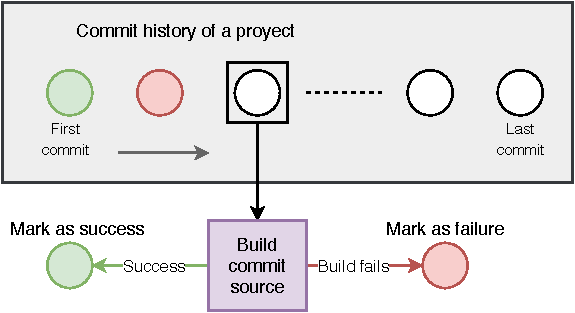
\includegraphics[width=\textwidth]{pages/01-Buildability/images/AnalysisProcess.pdf}
\caption{Process for checking compilability status of commits in a repository. ``Build commit source'' includes checking out the commit, checking for Maven configuration files, and if found, running Maven to try to build the code.}
\label{fig:commitHist}
\end{figure}

For each commit of interest in each repository, the script runs the following procedure (see also Figure~\ref{fig:commitHist}):
\begin{enumerate}
\item Check out the intended commit, obtaining the snapshot of the source code to be built.
\item Find the configuration for Maven (usually a \verb|pom.xml| file). If it is found, the build command for Maven is executed (\textit{mvn clean compile -X}) in a Docker container spawned for this specific analysis.
\item Collect the status code and the log produced by the execution in a log file (the verbose option of the command is used to obtain the most detailed log). If a configuration for Maven was not found, it is also noted in the log file.
\end{enumerate}

A further analysis of the log file allowed us to identify if the snapshot had configuration files for Maven, if the build was successful or not, and if not, the likely reason for the failure.

% jgb: SIZE. Remove next para if needed.
It is important to ensure the build environment is fully clean from results of previous builds, such as dependency modules or intermediate files that could influence the current one. To enforce this cleanup, besides the build command cleaning up local folders, the execution is encapsulated in a Docker container containing Maven and Java 8.

When checking for the presence of a Maven configuration file, we found an important replication issue: in all projects but three, those files were in exactly the same commits than the original study. But in those three, we found many more commits with Maven configuration (in the order of 6,000). We carefully inspected the checkout for a large sample of those commits, and our heuristics seem to work well. Unfortunately, this has some impact on the results of the replication, especially since a fraction of them are actually compilable. For having a more usable comparison with the results of the original study, we decided to analyze those commits separately (see details in Section~\ref{sec:buildability:results-repli}), so that the results on how compilability ``ages'' are not influenced because of them. That is the reason why the number of ``Commits (build conf.)'' in Table~\ref{table:statistics} is exactly the same (101,811) in both the original study (reduced) and our study (for the 79 considered repositories).

When searching for build files (pom.xml), we discovered that we were able to detect 4.72\% more commits with build files than the authors of the original study.
Detecting the presence of these build files is a relatively simple task, as they are easy to identify if they exist.
Nonetheless, to check if this inconsistency was due to an error in our scripts, we randomly selected a dozen commits where we found build files but the original study did not, and performed a manual inspection.
We found that our approach is the correct one.
So, probably the discrepancy is caused by some bug in the scripts of the original paper. As these scripts are not publicly available, we cannot confirm this possibility.

To explore the compilability of all of the snapshots, we used two Ubuntu 18.04 machines, one of them with 16 cores and 8 GB of RAM and the other one with 8 cores and 16 GB of RAM. The software we built was capable of balancing the load between both servers to minimize execution time, building several snapshots in parallel. Once the repositories to analyze were ready, the building of all snapshots took about four weeks of wall time to run.

\subsubsection{Obtaining Results}

The results of the study are obtained from analyzing the log file. From it, we can know if a Maven configuration was found for a commit, or if the build was successful. For the analysis on the causes of build failures, we analyze the exception produced by Maven from the log for the failed builds. The exceptions that can be produced during the construction of the Maven project are well defined and limited\footnote{https://cwiki.apache.org/confluence/display/MAVEN/Errors+and+Solutions}. For the reporting, we use the classification and mapping of exceptions in the original study, which defined four categories of errors: \textit{Resolution} (related resolution of artifacts, such as downloading of dependencies), \textit{Parsing} (such as malformed build configuration), \textit{Compilation} (during the compilation phase) and \textit{Other}. Note that the first three correspond to the first three steps in the building process described in~\cite{Sulir:2016:QSJ:3001878.3001882}, presented in Section~\ref{sec:buildability:related}.

For comparing our results with the original study, we also classified every commit according to how it behaved when building it in both studies:
%\begin{itemize}
\begin{inparaenum}[\bf(1)]
  \item \textbf{stable build}, the snapshot was built in both studies;
  \item \textbf{new error}, the snapshot was built in the original study, but not in ours;
  \item \textbf{same error}, the build failed in both studies for the same reason;
  \item \textbf{different error}, the build failed in both studies but for a different reason; and,
  \item \textbf{new build}, the build failed in the original study but not in ours.
\end{inparaenum}
%\end{itemize}

We tried to reproduce the methods of the original study as much as possible, using the same classification to enable a comparison as is mandatory in a replication study.
However, we did not do it manually but automated the procedure.
We took therefore advantage of the description of the Java exceptions used in their classification by the original authors in their reproduction package\footnote{http://www.cs.wm.edu/semeru/data/breaking-changes/}.
As each exception is mapped to exactly a single category, our tool took this mapping and applied it automatically, avoiding the necessity for a manual classification.
We think this highlights one of the main reasons for replication studies: to be able to detect and fix limitations in previous works.
Our tool and data sources are publicly available in our reproduction package.


\subsection{Reproduction study}

\subsubsection{Subject selection and recovery}

For our reproduction study, we generated a new dataset of repositories to analyze. Inspired by~\cite{Sulir:2016:QSJ:3001878.3001882}, we obtained a long list of repositories via the GitHub API, meeting the following criteria:

\begin{itemize}
\item \textit{Java as the programming language}. We wanted to check Java building technologies, staying in the same domain of the original study.
\item \textit{At least 500 stars and 300 forks}. We wanted some indicator of relevance.
\item \textit{At least five years of development}. We wanted to have a long enough commit history, so that the analysis was more complete.
\item \textit{Active in January 2020} (at least one commit). We wanted projects with recent activity, to include current practices.
\item \textit{Use a build system}. We wanted to check compilability, so we checked that they were using Maven, Gradle or Ant (the three most popular build systems for Java) in the last commit.
\item \textit{Between 1,000 and 10,000 commits}. We wanted to avoid projects too small, which would have few snapshots to analyze, but also very large ones, which would consume too many resources for the analysis.
\item \textit{No Android projects}. Because of a practical limitation: building projects for Android is in general more complex, and requires specific procedures.
\end{itemize}

From the long list meeting all these conditions, we randomly selected repositories for our reproduction study and proceeded to their analysis.
For each repository, we considered all commits in the master branch as the commits of interest for the study. 
A total of 80 projects have been selected for this reproduction study.
The total number of commits was 300,873.
When comparing the resulting list with the list of projects from the original analysis, in addition to variety (since the previous analysis was focused only in ASF projects), the main difference is that we focused in non-small projects with certain relevance.

\subsubsection{Building}

The process we followed to explore the buildability of snapshots for the repositories in our list was very similar to the one described above for the replication study. The differences were as follows:

\begin{itemize}
\item After checking out a commit, three systems are considered when searching for build configuration (see ``Build File'' in Table~\ref{table:buildSystems}). In the replication study only Maven was considered.
\item When building the snapshot with more than one build system, we tried the build systems in order: first Maven or Gradle, and if it failed, then Ant. We did not find snapshots with both Maven and Gradle. Having Ant and one of Maven or Gradle is usually due to the project transitioning from the former to the latter, thus still having the old Ant configuration and a new configuration for Maven or Gradle. Our order for testing systems considers that if the Maven or Gradle configuration worked, the project had likely already transitioned to them, if it did not, the project was still with Ant.
\item For each build configuration, we executed the build command defined by the build configuration (see ``Command'' in Table~\ref{table:buildSystems}).
\end{itemize}

\begin{table}[h]
  \caption{Build systems considered in the reproduction study}
  \label{table:buildSystems}
  \centering
  \begin{tabular*}{\textwidth}{@{\extracolsep{\fill}}lll}
    \toprule
    \bf{Build System} & \bf{Command} & \bf{Build File}\\
    \midrule
    Maven & mvn clean compile -X & pom.xml\\
    Gradle & ./gradlew build -x test & build.gradle \\
    Ant & ant compile  & build.xml \\
    \midrule
  \end{tabular*}
\end{table}
 
For this reproduction study, the Docker container we used included Java 8, Ant and Maven, while Gradle was run standalone (since it works self-contained). 
%Once the repositories to analyze were ready, 
The building of all snapshots took about two weeks of wall time, in the same environment we used for the replication study.


\subsubsection{Obtaining results}

As we did for the replication study, the results of the reproduction study are obtained by analyzing the logs of the attempts to build each considered commit from our list of repositories. The analysis is the same that we described already, with the difference that in the reproduction study we considered not only if the snapshot could be built or not, but also which build system was used. We also had to extend the mapping of exceptions in error logs to one of the four categories of errors in the original study (\textit{Dependency}, \textit{Parsing}, \textit{Compiling} or \textit{Other}). 
The new error mapping will be shown in the following sections, as well as being available in the reproduction package.


\section{Replication Study: Results}
\label{sec:buildability:results-repli}
% REPLICATION RESULTS

\subsection{Data for replication}

The original paper comes with a reproduction package, which we have found tremendously useful. It includes the complete list of commit hashes for all the analyzed repositories, and counts per repository of the main results. This allowed us to compute counts for our reduced set of 79 repositories. This way, we could do a fair comparison between the replication and the original results.

After computing our results for the 79 repositories in the original study, we found a discrepancy in the total number of commits. According to the original paper, 219,395 commits were analyzed. But computing from the list of commit hashes, we counted 174,505. To be consistent with other data in our study, which was extracted from that reproduction package, we used the second number in our tables. This fact does not impact the results, since we focus on the analysis of the reduced set of 79 repositories.

The scripts used for the original study are not available in its reproduction package. This is not a problem in itself, since we created our own software. But we could not determine the reason for some discrepancies, e.g., on the number of snapshots with build configuration (see details below). Maybe the heuristics coded into the original software took into account something that we missed, or maybe it didn't detect that configuration information in some cases.

Detailed logs of the execution are also not available in the reproduction package of the original study, making it difficult to explain some differences found in the compilability of a large number of commits in three repositories (see details below): we do not know if there was some error in the execution of the original study, or if we are missing something in our own.

\vspace{0.3cm}
\fbox{\begin{minipage}{0.9\textwidth}
\textbf{\textbf{RQ\textsubscript{1.1d}}: ``Is the data in the reproduction package of the original study enough for a replication?''} There is enough data for comparing results, even at the repository level. However, there is not enough data to exactly reproduce the original study: a copy of the git repositories, as they were when the analysis was performed, is missing; some relevant software is also missing (such as the one to detect the Maven configuration in a snapshot); and the logs of their execution for all snapshots is also missing, which makes it difficult to understand the reasons of some discrepancies when replicating the study.
\end{minipage}}

\subsection{Compilability}

To answer RQ\textsubscript{1.1a} and RQ\textsubscript{1.1c} in detail, we follow the same process as the original study, classifying repositories in three categories according to their number of commits: short history (number of commits in the first quartile, Q1), medium history (Q2 and Q3) and long history (Q4). Repositories classified as short (20) have less than 203 commits, medium (39 repositories) have between 203 and 1,148 commits, and long repositories (20) have more than 1,148 commits. Then, we analyze the compilability of those snapshots for which we found configuration for Maven, assuming the rest could not be built because developers were not using automatic tools for building.

Tables~\ref{table:replication-compilability} and \ref{table:replication-compilability-2} shows the results for compilability in the original study, and of our replication study. For the original study we computed, thanks to the details in its reproduction package, results for the reduced list of 79 repositories that we have analyzed. However, the results for the pristine study (with all its 100 repositories) are very similar to those of the reduced one. For example, the average compilability of the reduced study is 37.19, while for the pristine study it is 38.13, according to the original paper. For completeness, we run Wilcoxon's test on the compilability results of all projects of the previous and our replication studies, obtaining a p-value of 1.9077e-6. This confirms statistical significant differences between both cases.

% TABLE 1
\begin{table*}[h]
\caption{Compilable snapshots - Distribution (top: Reduced Original Study, bottom: Replication Study).}
%\label{table:originalResultsCompilability}
\label{table:replication-compilability}
\begin{center}
\resizebox{\textwidth}{!}{%
  \begin{tabular}{llllllll}
  \toprule
    \bf{Projects} & \multicolumn{7}{l}{Fraction built (in \%)} \\
                  & \multicolumn{7}{l}{} \\
                  & \bf{Min} & \bf{1st Qu.} & \bf{Median} & \bf{Mean} & \bf{3rd Qu.} & \bf{Max} & \bf{SD} \\  
  \midrule
  Short history  & 0.00     & 23.67        & 48.64       & 49.85      & 82.73       &  97.01   & 35.08 \\ 
  Medium history & 0.00     &  4.99        & 36.24       & 38.43      & 68.42       & 100.00   & 34.03 \\
  Long history   & 0.00     &  0.00        & 16.48       & 22.14      & 25.67       & 100.00   & 29.33 \\
  \midrule
  All            & 0.00     & 2.91         & 28.64       & \bf{37.19} & 66.00       & 100.00   & 34.25 \\ 
  \bottomrule
  \end{tabular}
}
\end{center}

\begin{center}
\resizebox{\textwidth}{!}{%
  \begin{tabular}{llllllll}
    \toprule
    \bf{Projects} & \multicolumn{7}{l}{Fraction built (in \%)} \\
                  & \multicolumn{7}{l}{} \\
                  & \bf{Min} & \bf{1st Qu.} & \bf{Median} & \bf{Mean} & \bf{3rd Qu.} & \bf{Max} & \bf{SD} \\  
  \midrule
  Short history  & 0.00     & 0.55         & 31.49       & 40.62      & 82.72        & 99.01     & 39.97 \\ 
  Medium history & 0.00     & 0.00         & 1.70        & 20.99      & 38.24        & 95.23     & 29.52 \\ 
  Long history   & 0.00     & 0.00         & 9.44        & 17.56      & 19.17        & 100.00    & 28.31 \\ 
  \midrule
  All            & 0.00     & 0.00         & 8.74        & \bf{25.1}  & 41.64        & 100.00    & 33.07 \\ 
  \bottomrule
  \end{tabular}
}
\end{center}
\end{table*}


%% TABLE 2
\begin{table*}[h]
  \caption{Compilable snapshots - Totals (top: Reduced Original Study, bottom: Replication Study).}
  %\label{table:originalResultsCompilability}
  \label{table:replication-compilability-2}
  \begin{center}
  
  \begin{tabular*}{\textwidth}{l|llllllll|lll}
  \toprule
    \bf{Projects} & \multicolumn{3}{c}{Total commits} \\
                  & \multicolumn{1}{c}{\bf{with build conf.}} & \multicolumn{1}{c}{\bf{Build success}} & \multicolumn{1}{c}{\bf{Fraction built}} \\
  \midrule
  Short history  &   2,311 &  1,129 & 48.85\% \\ 
  Medium history &  26,903 &  9,602 & 35.69\% \\
  Long history   &  72,597 & 12,006 & 16.54\% \\
  \midrule
  All            & 101,811 & 22,737 & 22.33\% \\ 
  \bottomrule

  \midrule
  Short history  &   2,311 &    876 & 37.91\%\\ 
  Medium history &  26,903 &  6,049 & 22.48\%\\ 
  Long history   &  72,597 &  7,739 & 10.66\%\\ 
  \midrule
  All            & 101,811 & 14,664 & 14.40\%\\ 
  \bottomrule
  \end{tabular*}
  \end{center}
\end{table*}



\vspace{0.2cm}
\fbox{\begin{minipage}{0.9\textwidth}
\textbf{ \textbf{RQ\textsubscript{1.1a}}: ``How many snapshots from the change history are compilable?''} 8.74\% or less of the commits were compilable for half of the analyzed projects. The result for the original study was 28.64\%.
Thus, results are very different, likely affected by the time passed (as we will discuss when answering RQ\textsubscript{1.1c}).
\end{minipage}}

\fbox{\begin{minipage}{0.9\textwidth}
\textbf{\textbf{RQ\textsubscript{1.1c}}: ``Has compilability degraded since the original study?''}
A much smaller fraction of the commits with build configuration can be built (22.33\% in the original study versus 14.66\% in our replication). When analyzing repositories by size, medium projects are more affected by this decrease in compilability, with half of them having a compilability of 1.70\% or less, while in the original study that number was 36.24\%. Short projects are also affected, and the less affected are long projects, but still they move from a median of 16.48\% to 9.44\% in our replication.
\end{minipage}}
\vspace{0.2cm}

We found significant differences in three repositories when checking for the existence of Maven configuration files (for all the others, results are exactly the same). In those three repositories we found 6,583 extra commits with a Maven configuration. When trying to build them, we could build 442 extra snapshots, which would increase the number of compilable snapshots to 15,106 (from a total of 108,394), or 13.93\% compilability, slightly less than 14,40\, as shown in Table~\ref{table:replication-compilability-2}.

We also checked all snapshots for configuration files of Ant and Gradle (we only found for Ant), finding 2,586 additional snapshots that could be built, leading to a total of 17,692 commits built. However, these results are not comparable with the original study, since they did not consider Ant.

Table~\ref{table:replication-buidability-summary} summarizes the results of all replications, with the different cases.
It should be noted that Table~\ref{table:replication-compilability} extends the information of the results reported in the ``Replication'' row of Table~\ref{table:replication-buidability-summary}, as it is the most comparable scenario between the original and the replication study.

\begin{table*}[h]
\caption{Original and replication studies (Summary of results). Replication\textsubscript{a}: use same build configs, Replication\textsubscript{b}: use all detected Maven config files, Replication\textsubscript{c}: use all detected Maven and Ant config files}
\label{table:replication-buidability-summary}
\resizebox{\textwidth}{!}{%
  \begin{tabular}{lrrrrrr}
  \toprule
  & Repos.                        & All     & Commits           & Commits & Built & Built \\
  &                              & Commits & w/build conf    & built   & total          & mean of\\
  &                              &         &                   &         &                & projects \\
  \midrule 
  Pristine Original               & 100     & 174,505 & 132,484 & 31,696  & 23.92\%        & 37.74\% \\
  Reduced Original                &  79     & 139,389 & 101,811 & 22,737  & 22.33\%        & 37.19\% \\
  Replication\textsubscript{a}    &  79     & 139,389 & 101,811 & 14,664  & 14.40\%        & 25.09\% \\
  Replication\textsubscript{b}    &  79     & 139,389 & 108,394 & 15,106  & 13.93\%        & 25.42\% \\
  Replication\textsubscript{c}    &  79     & 139,389 & 117,124 & 17,692  & 15.10\%        & 24.85\% \\  
  \bottomrule
  \end{tabular}
}
\end{table*}


\subsection{Failure analysis}

To answer RQ\textsubscript{1.1b}, and provide some insight on the reasons for the answer to RQ\textsubscript{1.1c}, we analyzed build failures following the categorization of the original study. Table~\ref{table:allCauses} reports the classification results for the previous study and for our replication, in both cases for the 79 repositories of the reduced study.

\begin{table}[h]
\caption{Causes of failed builds.}
\label{table:allCauses}
\begin{center}
\begin{tabular*}{\textwidth}{@{\extracolsep{\fill}}rrrrr}
\toprule
\multicolumn{1}{l}{}	    & \multicolumn{2}{c}{\bf{Original study}}    & \multicolumn{2}{c}{\bf{Replication study}}  \\
\bf{Categories}                 & \multicolumn{1}{r}{\#} & \multicolumn{1}{r}{\%} & \multicolumn{1}{r}{\#} & \multicolumn{1}{r}{\%}  \\
\midrule
Resolution  & 47,832 &  60.49 & 55,299 & 63.45  \\
Parsing     &  9,595 &  12.13 & 10,350 & 11.88  \\
Compilation &  2,807 &   3.55 &  2,544 &  2.92  \\
Other       & 18,839 &  23.83 & 18,954 & 21.75  \\
\midrule
All errors & 79,073 & 100.00 & 87,147 & 100.00 \\
\bottomrule
\end{tabular*}
\end{center}
\end{table}

Table~\ref{table:causesDetailed} shows the changes we observed when building snapshots with respect to the original study, according to the classification provided in Section~\ref{sec:buildability:metodology}. We could build 14,480 (63.68\%) of the successful builds in the original study (\textit{stable builds}). We could also build some snapshots that could not be built in the original study. In general, these correspond to external artifacts that were not available when they run their experiments, but were available when we run ours. These \emph{new build} snapshots amount to 184 (0.13\%).

% jgb: Keeping this old table, with only errors, in case we need to
% revert to it because of size limits (and write the data about new and
% stable builds somewhere else
%
% \begin{table}[]
% \caption{Changes in causes of failed builds}
% \label{table:causesDetailed}
% \begin{tabular}{rrrrrrr}
% 	\toprule
% \multicolumn{1}{l}{\bf{Categories}} & \multicolumn{2}{c}{\bf{Same error}} & \multicolumn{2}{c}{\bf{Different error}} & \multicolumn{2}{c}{\bf{New error}} \\
% \bf{(Replication)} & \multicolumn{1}{c}{\#} & \multicolumn{1}{c}{\%} & \multicolumn{1}{c}{\#} & \multicolumn{1}{c}{\%} & \multicolumn{1}{c}{\#} & \multicolumn{1}{c}{\%} \\
% \midrule
% Resolution & 42,826  & 49.14  & 4,704 & 5.39  & 4,868  & 5.59                    \\
% Parsing                & 9,485                   & 10.88                   & 694                     & 0.79                    & 171                     & 0.20                    \\
% Compilation            & 2,544                   &  2.91                   & 0                       & 0.00                    & 0                       & 0.00                    \\
% Other                  & 12,443                  & 14.27                   & 6,194                   & 7.10                    & 3,218                   & 3.69                    \\
% \midrule
% All errors & 67,298 & 77.22 & 11,592 & 13.30 & 8,257 & 9.48 \\                 
% \bottomrule
% \end{tabular}
% \end{table}

\begin{table}[]
\caption{Changes in builds (original to replication).}
\label{table:causesDetailed}
\centering
\resizebox{\textwidth}{!} & \multicolumn{1}{c}{\#} & \multicolumn{1}{c}{\%} & \multicolumn{1}{c}{\#} & \multicolumn{1}{c|}{\%} & \# & \# \\
  \midrule
  Resolution             & 42,826                  & 49.14                   & 7,605                   & 5.39                    & 4,868                   & 5.59                    \\
  Parsing                & 9,485                   & 10.88                   & 694                     & 0.79                    & 171                     & 0.20                    \\
  Compilation            & 2,544                   &  2.91                   & 0                       & 0.00                    & 0                       & 0.00                    \\
  Other                  & 12,443                  & 14.27                   & 3,293                   & 7.10                    & 3,218                   & 3.69                    \\
  \midrule
  All  & 67,298 & 77.22 & 11,592 & 13.30 & 8,257 & 9.48 & 14,480 & 184 \\ 
  \bottomrule
  \end{tabular}
}
\end{table}

For 67,298 of the snapshots that failed to build, we reported the same exception as in the previous experiment (\textit{same error}). Therefore, adding these to \textit{stable build}, 81.778 (80.66\% of the snapshots with build configuration) behaved exactly as in the original study. On the other hand, for 13.30\% of the snapshots that failed for us, we found a different error than in the original study (\textit{different error}), while 9.48\% of the snapshots that failed for us did not fail in the original study (\textit{new error}).

Both in \textit{different error} and in \textit{new error}, one of the main causes for failed builds is \textit{Resolution}, and specifically, the resolution of external artifacts needed for the build. We can affirm that one of the main reasons for the degradation in compilability with time is the impossibility of recovering more and more of the dependencies of these projects as time passes. On the other hand, \textit{Compilation} errors only appear in \textit{same error}, since they only depend on using the same compiler (so if they failed in the replication, they should have failed in the original study). Comparing the number of \textit{Compilation} errors in the replication and in the original study, it decreased from 2,807 to 2,544. Some inspection raised the cause: new exceptions mask previous building errors.

% jgb: SIZE We could remove the next para if needed
We studied in some detail the \textit{Resolution} category. One of the most recurrent cause was experiencing timeouts when accessing some external artifact, usually a dependency (5.12\% of total errors). This type of error appears only as \textit{different error} or \textit{new error}. Given that no long network failures were observed during the execution of our study, this is due to access to artifacts that are no longer available, which is consistent with the previous comment on dependencies.

\vspace{0.2cm}
\fbox{\begin{minipage}{0.9\textwidth}
\textbf{\textbf{RQ\textsubscript{1.1b}}: ``What types of errors prevent snapshots from being built?''}
The proportion of the different kinds of errors is similar to the original study. Most of the errors (63.45\%) are caused by resolution of dependencies and other external artifacts (60.49\% for the original study), these being the errors that contributed the most to the degradation of compilability. Parsing errors convey 11.88\% of the failures we detected, close to the 12.13\% reported in the original study. The same can be said for Compilation errors (2.92\% in our replication \emph{vs.} 3.55\% in the original study). About 80\% of the snapshots behaved exactly like in the previous study (they built, or they failed with the same error).
\end{minipage}}


\section{Reproduction Study: Results}
\label{sec:buildability:results-repro}
% REPRODUCTION RESULTS

\subsection{Compilability}

To answer RQ\textsubscript{1.2a}, we repeated the same analysis of the replication study, but now for the 80 projects of our reproduction study. Of them, 20 projects were classified as having a short history (Q1, less than 1,974 commits), 40 as medium history (Q2 and Q3), and 20 as long history (Q4, more than 4,847 commits). Compilability results are shown in Table~\ref{table:results-reproduction}.

\begin{table*}[h]
\caption{Reproduction study - Compilability results}
%\label{table:ourResultsCompilabilityReproduction}
\label{table:results-reproduction}


% TABLE 1
\begin{center}
\resizebox{\textwidth}{!}{%
  \begin{tabular}{@{\extracolsep{\fill}}l|lllllll|lll}
  \toprule
    \bf{Projects} & \multicolumn{7}{c}{Fraction built (in \%)} & \multicolumn{3}{c}{Total commits}\\
    \bf{by history} & \multicolumn{7}{c}{} & \bf{with} & \bf{Build} & \bf{Fraction} \\
                  & \bf{Min} & \bf{1st Qu.} & \bf{Median} & \bf{Mean} & \bf{3rd Qu.} & \bf{Max} & \bf{SD} & \bf{build conf.} & \bf{success} & \bf{built}\\   
  \midrule
  Short          & 0.00     & 37.43        & 55.42       & 58.21          & 82.27 &  99.38 & 28.12  & 28,312 & 15,948 & 56.32\%\\
  Medium         & 0.00     & 10.56        & 34.94       & 40.35          & 68.60 & 100.00 & 33.34 & 114,716 & 44,688 & 38.96\%\\
  Long           & 0.00     & 4.27        & 12.80       & 27.76          & 48.04 &  93.52 & 31.76 & 138,459 & 37,852 & 27.33\%\\
  \midrule
  All            & 0.00     & 10.56        & 36.25       & \textbf{41.66} & 70.62 & 100.00 & 33.18 & 281,487	 & 98,488	 & 34.98\%\\
  \bottomrule
  \end{tabular}
}
\end{center}

% % TABLE 2
% \begin{center}
% \begin{tabular*}{\textwidth}{@{\extracolsep{\fill}}l|lll}
% \toprule
%   \bf{Projects} & \multicolumn{3}{c}{Total commits} \\
%                 & \multicolumn{1}{c}{\bf{with}} & \multicolumn{1}{c}{\bf{Build}} & \multicolumn{1}{c}{\bf{Fraction}} \\
%                 & \bf{build conf.} & \bf{success} & \multicolumn{1}{c}{\bf{built}}\\    
% \midrule
% Short history  & 28,312 & 15,948 & 56.32\%\\
% Medium history & 114,716 & 44,688 & 38.96\%\\
% Long history   & 138,459 & 37,852 & 27.33\%\\
% \midrule
% All            & 281,487	 & 98,488	 & 34.98\%\\
% \bottomrule
% \end{tabular*}
% \end{center}

\end{table*}

% TABLE 3

\begin{table*}[h]
  \caption{Reproduction study - Compilability by build system.}
  \label{table:results-reproduction-build-systems}

\begin{center}
  \begin{tabular*}{\textwidth}{@{\extracolsep{\fill}}l|rrr}
  \toprule
  \bf{BuildSystem} & \multicolumn{3}{c}{Compilability}                                  \\
  \bf{}	& \bf{\#Commits} & \bf{\#Build success} & \bf{Fraction built} \\
  \midrule
  Maven           &        191,063  &                     80,310 &            42.03\%  \\
  Ant             &         25,735  &                      4,441 &            17.26\%  \\
  Gradle          &         64,095  &                     13,737 &            21.43\%  \\
  \midrule
  All             &        280,893  &                     98,488 &            35.06\%  \\
  \bottomrule
  \end{tabular*}
\end{center}

\end{table*}

% TABLE 4

\begin{table*}[h]

  \caption{Reproduction study - Errors by build system.}
  \label{table:results-reproduction-build-systems-errors}

\begin{center}
\resizebox{\textwidth}{!} & \bf{\#} & \bf{\%}  & \bf{\#} & \bf{\%}  & \bf{\#} & \bf{\%} \\
  \midrule
  Maven           &          75,806 &             68.45\%  &        1,967 &            1.78\% &                0 &                0.00\% &     32,980 &        29.78\% \\
  Ant             &           4,485 &             21.06\%  &            0 &            0.00\% &            1,077 &                5.06\% &     15,732 &        73.88\% \\
  Gradle          &          22,260 &             44.20\%  &            0 &            0.00\% &            2,373 &                4.71\% &     25,725 &        51.08\% \\
  \midrule
  All             &         102,551 &             56.22\%  &        1,967 &            1.08\% &            3,450&                1.89\% &     74,437 &        40.81\% \\
  \bottomrule
  \end{tabular}
}
\end{center}

\end{table*}

For all categories, and for all the projects together, median and mean are close, meaning the distribution is not very skewed: to some extent we were successful in avoiding bias when selecting projects to analyze.  
The standard deviation shows a large spread in the values (compatible with the values observed for the different quartiles). 
The fraction of snapshots that could not be built in all categories is higher than (or very close to) 50\%, which shows that automatic compilability of past snapshots can certainly not be given for granted. 
Projects with a long history have in general less compilability, and compilability increases as we move to projects with a medium and short history.

It should be noted that in the original study, we found a great diversity in the size of the projects according to their number of commits (from projects with 25 commits to 14k).
The problem with smaller projects ($<$203 commits) is that in many cases they have not had a natural development (the initial commit imports code from another source, as can be seen for example in following commit\footnote{https://github.com/apache/maven-app-engine/commit/b77ad9e82d7cc94}).
This means that part of the project's development history is lost, which is a limitation of the original study.
In the selection criteria for the repository mining we have taken this limitation into account, setting a lower limit of 1000 commits.
Because of this difference between experiments, the separation between small, medium and large projects is different and the groups cannot be compared between experiments. 
Nonetheless, for the sake of completeness, we offer a comparison using the same quartiles to classify the projects into the three categories in a table that can be found in the replication package.

\vspace{0.2cm}
\fbox{\begin{minipage}{0.9\textwidth}
\textbf{\textbf{RQ\textsubscript{1.2a}}: ``How many snapshots from the change history are compilable?''}
Less than half of the snapshots with build configuration could be built. Compilability decreased with the size of the commit history of projects. For all history size categories, and all projects together, mean and median compilability was less than 51\%, although variability is high (standard deviation is over 28\% in all cases).
\end{minipage}}

\subsection{Failure analysis}

To answer RQ\textsubscript{1.2b}, we analyzed build failures, as shown in Table~\ref{table:results-reproduction-build-systems-errors}. Most of the errors are of type \textit{Resolution}, due to missing dependencies and other external artifacts. \textit{Parsing} and \textit{Compilation} errors are almost negligible.

% \begin{table}[h]
% 	\caption{Causes of failed builds (Reproduction Study)}
% 	\label{table:resultsGithub}
% 	\begin{center}
% 	\begin{tabular}{rrr}
% 		\toprule
% 		\bf{Action}  & \bf{\#} & \bf{\%} \\
% 		\midrule
% 		Resolution      &  32,671   &  56.32 \\
% 		Parsing         &     970   &   1.67 \\
% 		Compilation     &   1,248	&   2.15 \\
% 		Other           &  23,125   &  39.86 \\
% 		\midrule
% 		All            &   58,014   & 100.00 \\
% 		\bottomrule
% 	\end{tabular}
% 	\end{center}
% \end{table}

The fact that most errors are due to missing external objects is a good indicator of further decline of compilability in the future: as time passes, more and more artifacts will disappear, which will lead to more and more commits not building. The low numbers for \textit{Parsing} and \textit{Compilation} errors are interesting: they could be indicating that the use of automatic tools to check the compilability of snapshots (and therefore, the consistency of building configuration, and the correctness of compilation) before merging the corresponding commits.

\vspace{0.2cm}
\fbox{\begin{minipage}{0.9\textwidth}
\textbf{\textbf{RQ\textsubscript{1.2b}}: ``What types of errors prevent snapshots from being built?''}
Most of the errors observed (56\%) are due to missing dependencies and other external artifacts. The impact of these errors in the overall compilability is thus very important: almost one third (36.43\%) of all snapshots with building configuration could not be built because of them. However, parsing and compilation errors are few, meaning that most snapshots were carefully checked for these errors before committing.    
\end{minipage}}


\subsection{Building system}

To answer RQ\textsubscript{1.2c}, we performed an analysis by build system. When we were detecting build configuration files, we observed some projects starting to build with Ant, then switching to Maven or Gradle, and some others using Maven and Gradle for their entire history. From the total number of commits with build configuration, 68.02\% are for Maven, 22.82\% for Gradle, and 9.16\% for Ant. The results of the analysis by build system are shown in Table~\ref{table:results-reproduction-build-systems}.

The first interesting result is that compilability for snapshots with Maven is much higher (42.03\%) than for Ant or Gradle (17-22\%). With respect to specific kinds of errors, Maven is dominated by \textit{Resolution}, as Gradle and Ant is dominated by \textit{Other}. However, the sample of snapshots with Ant and Gradle is relatively small, which means our results for them are less reliable.

The detailed classification of errors for all building systems can be found in the Table~\ref{table:other-errors} (The table is limited to the 20 most frequent errors, the full table can be found in the reproduction package). 
From this classification, it is worth mentioning:
\begin{itemize}
 \item From the 15,732 \textit{other errors} for Ant, 8,615 are failures because they do not have the ``compile'' task defined (which is a standard in the development of projects with Ant), and about 4,610 because a specific binary or config file is expected in the path, instead of being included as a dependency.
 \item From the 25,725 \textit{other errors} for Gradle, 5,215 of them fail because of a test that cannot be automatically ignored. A common error (4,726) is that some tasks, defined as scripts in the configuration file by the developer, fail to build the project. Other less common errors are the absence of a secret key (which is not usually stored in a public repository), an error in the generation of documentation or the lack of permissions for certain system folders. These errors, although a priori generic, are usually concentrated in a single project and are not significant.
\end{itemize} 

Although all of these snapshots could not be built automatically, they could be built with minimal human intervention, or with a slightly improved set-up of the build configuration for the projects affected. Given the relatively small sample of snapshots for these two systems (Ant and Gradle, compared to Maven), considering these snapshots as errors or not would change dramatically the figures for the \textit{other errors} category for both of them. In the reporting of results, we have decided to consider those cases as errors, which is a cause for the lower compilability reported for Ant and Gradle.

\newpage

\begin{table}[]
  \caption{Classification of errors for all build systems}
  \label{table:other-errors}
\resizebox{\textwidth}{!} \\ \hline
  Maven                & ArtifactResolutionException        & Resolution      & 74,950          & 41.09       \\ \hline
  Maven                & MojoFailureException               & Other           & 12,426          & 6.81        \\ \hline
  Maven                & MojoExecutionException             & Other           & 11,562          & 6.34        \\ \hline
  Ant                  & Target "compile" does not exist    & Other           & 8,615           & 4.72        \\ \hline
  Gradle               & IOException: Server returned ...   & Resolution      & 8,057           & 4.42        \\ \hline
  Gradle               & Could not resolve                  & Resolution      & 7,057           & 3.87        \\ \hline
  Gradle               & Could not resolve all dependencies & Resolution      & 6,899           & 3.78        \\ \hline
  Maven                & ConnectException                   & Other           & 5,524           & 3.03        \\ \hline
  Gradle               & Task 'test' not found              & Other           & 5,215           & 2.86        \\ \hline
  Gradle               & Execution failed for task          & Other           & 4,726           & 2.59        \\ \hline
  Gradle               & Cannot run program                 & Other           & 4,540           & 2.49        \\ \hline
  Ant                  & UnknownHostException               & Resolution      & 3,918           & 2.15        \\ \hline
  Gradle               & Other Gradle error                 & Other           & 3,849           & 2.11        \\ \hline
  Ant                  & Unable to find property file       & Other           & 3,693           & 2.02        \\ \hline
  Gradle               & Permission denied                  & Other           & 2,295           & 1.26        \\ \hline
  Gradle               & Compilation failed                 & Compilation     & 2,288           & 1.25        \\ \hline
  Maven                & PluginDescriptorParsingException   & Parsing         & 1,591           & 0.87        \\ \hline
  Gradle               & Could not find                     & Other           & 1,405           & 0.77        \\ \hline
  Ant                  & Other Ant error                    & Other           & 1,181           & 0.65        \\ \hline
  Gradle               & git-lfs is required to build       & Other           & 1,083           & 0.59        \\ \hline
  Ant                  & Compile failed                     & Compilation     & 1,077           & 0.59        \\ \hline
  \end{tabular}
}
\end{table}

\vspace{0.2cm}
\fbox{\begin{minipage}{0.9\textwidth}
\textbf{\textbf{RQ\textsubscript{1.2c}}: ``Are there differences in compilability depending on the building tool?''}
The compilability observed in commits whose build system is Maven is twice as high as that obtained for Gradle and Ant. Resolution errors are dominant for Maven (68.45\%), parsing errors are very low (1,96\% for Maven and 0\% for Ant and Gradle), and compilation errors seem to be only relevant for Ant (5.06\%, 4.71\% for Gradle, 0\% for Maven). We note that both Ant and Gradle use user-written tasks or scripts that are subject to errors, mainly because they do not follow tool standards, which negatively affects their compilability.
\end{minipage}}


 

\section{Discussion}
\label{sec:buildability:discussion}
When performing our studies, we wanted to learn about the validity of the results presented in~\cite{tufano2017there}, by checking how they had changed after about six years, and about their generality, by doing a similar analysis on a different set of projects. As a side result, we also expected to learn about conditions for the replication of this kind of studies, based on its very detailed reproduction package. We discuss our findings in the next subsections.

\subsection{Reproduction package}

The data in the reproduction package was not enough for a complete replication, although it helped substantially. The lists of repositories analyzed, commit hashes, and results per project were certainly the most useful data for us. With the list of repositories we could search for them in the ASF git repositories, in GitHub, and in Software Heritage. The list of hashes was fundamental for checking if those commits were still recoverable from any of these sites and the list of results per project was fundamental to compare with the original results once we decided to analyze only a part of the repositories in their analysis.

However, we also missed some data. In our search, we could not find some repositories. For 25\% of them we could not find all commits. Since git repositories may disappear, or commits in them can be removed, having a copy of the git repositories as they were analyzed would have allowed us for a complete reproduction. For the number of repositories analyzed, this is a massive dump, but small enough to be preserved in sites like Zenodo, which admits very large datasets. Software Heritage is also a very interesting option. At the time of the original study, they were still starting. But now, they are already archiving probably all code of interest for this kind of studies, and they are open to archive more if needed. Since they preserve all changes to the repositories they track, all commits studied will be available for future research.
Unfortunately, these types of problems we have encountered pertain to any study involving the analysis of a project's history. Kalliamvakou et al.~\cite{kalliamvakou2016depth} identified many perils that can be encountered when mining software repositories that are important to consider when conducting MSR-like studies. 
However, they do not include the perils that we have encountered, which negatively affect the replication of these studies. 
Future lists of perils should include those that affect the integrity of the repository over time:
\begin{itemize}
    \item The repository may no longer be accessible (it has been deleted or made private).
    \item Commits have been deleted
\end{itemize}

We also missed the software used for building the snapshots. Even when the methodology is clearly explained, we expect some details to be only available by reading the software. The lack of it prevented us from determining with certainty if the discrepancies in the number of builds for some repositories were due to errors in the original software, or in ours. For the same reason, we missed the logs of the original experiments. With them, we could have determined with more detail some of the discrepancies we found.

% jgb: SIZE A part of this could be removed if shortening the paper is needed
In summary, we recommend to include the following items in the reproduction package for this kind of studies: references to the repositories, list of commits, complete copy of the repositories, or references to the analyzed commits in Software Heritage, results at the finer grain possible (at least at the level of repositories), a copy of the software used (at least for the building of the commits), and a copy of the logs of executing it. Our reproduction package (see ``Acknowledgments and reproducibility'', at the end of this paper) includes all of these artifacts, plus the software used for the calculation of the results (as Python notebooks), with intermediate results. All of this is provided for both the replication and the reproduction studies.

\subsection{Replication study}

We have found less compilability than the original study. Some dependencies cease to be available with time, and as time passes, more and more of them are missing, impacting on the compilability of more and more snapshots. This depends on the kind of dependencies: official packages, in the case of Maven, are usually preserved. However, we have found many cases of specific links, or interim packages, that are much less reliable. We think this fact shows the importance of building strong configuration files for the build tools, that are designed to be resilient to the passing of time. Including references to artifacts that will be preserved (including, but not limited to, dependencies) as much as possible is an important part of it.
However, other errors due to compilation, parsing, etc., have remained stable, as it seems reasonable, because we are using basically the same tools for building the source code.

The length of the history in commits seems to have an impact on the changes from the original study to our replication. Projects with medium histories went from a median of about 36\% of built commits, to almost 0\% (1.7\%). We do not know if this is due to something specific in the sample of projects, or if there is some effect worth researching. It is also noticeable how the standard deviation of the distribution of built commits per project remains very stable.   

The overall numbers for compilability are rather small. For half the projects analyzed, less than 10\% of the commits can be built, which for practical purposes means most of the history of the project cannot be built automatically. This leads to an interesting detail: we have tried to build snapshots automatically, but maybe a manual approach --looking at the specific errors and trying to fix them-- could reach a much better overall compilability. However this approach, although interesting, is not of much practical use in many of the common scenarios in industry.

\subsection{Reproduction study}

The main reason for the reproduction study was to explore if the results of the original study were extensible to other, more diverse, Java programs. From the point of view of compilability, our results show only a partial extensibility. Mean compilability of projects is relatively similar (41\% in our reproduction, 37\% in the original study). Maybe the main conclusion is that a large number of snapshots in both cases are not compilable (clearly more than half, in both cases), showing the difficulties of past compilability.

When considering the kinds of errors leading to failed builds, it is clear in both studies the importance of \textit{Resolution} errors: about 60\% of all errors in the original study, 56\% in our reproduction. Both studies offer similar results for \textit{Compilation} errors: about 4\% and 2\%. We can conclude that the most influential errors, at least in the case of Java, are indeed \textit{Resolution}, and that \textit{Compilation} errors are not significant. Therefore, if a project wants to work on improving their past compilability, they should very likely work on improving the preservation of external artifacts, and on using references with guaranteed future availability. Clear rules could be derived, to ensure better configuration files for building tools, not degrading compilability as time passes. There is, however, little to do by the compiler to improve the situation, maybe due to the good work that Java does in ensuring backwards compatibility, or to the pre-merge testing that is usually done before producing new commits. These results are also in line with those discussed in the original paper.

We also studied the impact of different build systems on past compilability, which was not done in the original analysis. In our sample, we can say that snapshots using Maven show in general better compilability (about 42\%, as opposed to 17\% and 21\% for Ant and Gradle). The numbers for Ant could be underestimated in our study, as we explained, but the numbers for Gradle seem clear, despite the smaller sample of Gradle snapshots. A more extensive study should be performed to know if this is really a difference between the systems, or just a particularity of our sample.

\subsection{Mitigation measures}

The large number of errors that occur when trying to build commits from the past leads us to think about what possible measures we can take to reduce their occurrence. In the literature we find a large amount of Automatic Repair work that could solve some of the problems we are facing. In this section we will highlight two works that directly address build errors in previous snapshots, which will help us to make some recommendations to mitigate build errors.

Vassallo et al.~\cite{vassallo2020every} summarize the reasons why Maven builds fail and suggest possible solutions. The work includes a survey on how do developers approach different types of build failures. They consider dependency resolution issues to be the most difficult to address. Among the most difficult bugs to address are infrastructure bugs (entirely related to the execution context) and dependency resolution bugs. The former are not a problem in our case, as most projects that are mined from GitHub tend to be programming libraries. The latter are the most numerous in our experiments and highlight that the logs usually do not give much information about the error.

Macho et al.~\cite{macho2018automatically} propose a more specific tool focusing on problems related to Maven dependencies. Their study on how developers tend to fix dependencies themselves shows that in most cases it is usually enough to make a version number increase or promote a version with the -SNAPSHOT suffix to a stable version. Among the strategies of the tool we can find: Version Update (based on the usual behavior followed by the developer), Dependency Delete (deleting a problematic dependency that is no longer needed for the project), and Add Repository (in many cases, the configuration of the repository to which the artifacts are to be requested is not registered in the code repository, a possible fix being to add this artifact repository to pom.xml).

Based on the information from previous work and our experience in analyzing the results of the experiments we have conducted, we state possible mitigations for the problems that prevent a snapshot from being built. We want to approach these mitigations from two points of view: i) \textit{the developer} (who must consider that in the future he may need to re-build a particular version of his code, for example to include a patch), and ii) \textit{the researcher} (who performs experiments on the commit history of a project):

\begin{itemize}
    \item \textbf{Dependency resolution}: These errors represent a significant number for all three building systems. In some cases the dependencies are not from an artifact repository, but require manual installation within the project, or we may find authentication errors as the repositories are private. Developers should ensure that changes uploaded to the code repository include stable versions of the libraries for subsequent download from the artifact repositories. In the case of needing an additional resource (e.g., a library compiled directly to a JAR executable file), this should be versioned along with the rest of the code so that the code repository is self-contained. So, we have found SNAPSHOT errors because a project is multi-module and some modules depend on build versions from other modules (as it is the case for io.spring.initializr:initializr-generator-spring:jar:0.8.0.BUILD-SNAPSHOT). Researchers can mitigate some of the errors, for example, by removing the -SNAPSHOT suffix or replacing the library version with the version set by the next commit history where the build does work.
    \item \textbf{Parsing}: The main mitigation measure for this type of errors is usually the encoding. We have found non-English characters in code comments (usually author names) that prevent compilation. Developers should make sure that the encoding is present in the project configuration file, so that it is taken into account when building the project. Researchers can check if this configuration exists and overwrite it if it is not correct; or if they cannot find it, they can try to use the most inclusive encoding possible.
    \item \textbf{Compilation}: These errors are often due to code that has been commented out and that simply cannot work and needs to be manually inspected, sometimes with some knowledge of the project's operation. In previous work, Tufano et al. considered that there were builds that were broken from conception; compilation bugs often fall into this category. Therefore, we have not established any mitigation measures for this type of bugs.
    \item \textbf{Other}: Errors in this category include all those that do not fit into any of the above categories. 
    In the case of Gradle and Ant, this is the predominant category. 
    In these build systems, unlike in Maven, it is the developer who defines through tasks or scripts the steps to be carried out to build the project. 
    This can make it very difficult to automate the build if the developer has not used the standard tasks of the build system and has defined his own tasks (which can be subject to errors). Some of the most recurring errors encountered are: \emph{Target ``compile" does not exist} (Ant), \emph{Task `test' not found} (Gradle), and \emph{Execution failed for task X} (Gradle). 
    Developers should use standard task names. 
    It is common that after a while another developer has to build a past version of the code and tries to build the project using standard tasks. 
    Researchers should consider that at some points in the project, standard task names may not be used. 
    The documentation can help in understanding how the project should be built, and if that fails, Continuous Integration (CI) configuration files can be inspected as they usually contains these build commands correctly versioned alongside the code.
\end{itemize}


\subsection{Threats to validity}

Our studies are subject to construct validity issues, mostly due to how we define compilability of a snapshot (the snapshot is automatically compilable now, using only the available source code in the snapshot). The usual compilability is defined not for past commits, but for the current ones, but we are interested specifically in the case of building commits in the history of the project. In addition, it could be argued that a snapshot could be built with more advanced techniques (e.g., by extracting the build command from the documentation or, failing that, from the CI files), or by fixing by hand some of the errors. However, we were specifically interested in the automatic case, and we think the techniques we used for building are the usual ones.

Our results are also subject to internal validity issues, mainly because of our interpretation of what an error is, and to the specific heuristics that we use to detect and classify build failures. Also, to any kind of bug in our execution or analysis software. We make this information available in the reproduction package, so that these issues can be inspected.

Threats to conclusion validity could come from our interpretation of the results. We think that our statistical methods and interpretations are the usual ones. Just in any case, we share the Python notebooks we have used, so that they can be inspected.

Finally, we can also have external validity issues. We think we have at least partially mitigated those mentioned in the original paper, by generalizing results replicating the analysis, and performing the reproduction analysis with a more diverse and different dataset. Still, we have concerns of how general these results are for Java projects, even when they are coincident with the original study. Extension to other languages is still a matter of further research.


\section{Conclusions and future Work}
\label{sec:buildability:conclusions}
In this chapter we have shown a replication and a reproduction study from Tufano et al. work~\cite{tufano2017there} about the compilability of the history of past commits of a project. In the first one we have repeated their analysis, with those repositories for which we found all commits, and in the second one we extended its generality by using the same methodology with a different, more diverse set of Java projects, and considering also Ant and Gradle in addition to Maven.

The main contributions of this work are:

\begin{itemize}
\item A discussion and guidelines on reproduction packages for studies on the compilability of past snapshots. 
\item A dataset and software, usable by other researchers, to study long-term degradation of compilability.
\item A partial validation of the results of the original study. In particular, results about frequency of errors causing build failures have been validated and extended.
\item Evidence on how compilability degrades over time, and how it could be mitigated by ensuring future availability of dependencies.
\item Evidence on the compilability of a different, more diverse set of Java projects, showing some differences with the original study.
\item Evidence on how the building tools affect future compilability.
\end{itemize}

%\grex{Lo he dejado así}
%:\jgb{Lo he retocado un poco}
In summary, we wanted to shed some more light on to which extent past snapshots of projects are compilable ``as such'', because that is the basis to know how much build-repair techniques are needed if past artifacts of a project need to be reproduced from source code.
Since our study was a replication and a reproduction, a part of our results could be expected, but still they add more detail and evidence to the original study. In addition, we also found some differences, generalized evidence by analyzing a more diverse set of projects, and produced a tool to automate the analysis of any Java repository, which could be used in further studies by any researcher.

Still, more research is needed to draw general conclusions on the compilability of past snapshots, especially for languages other than Java, to get a more precise knowledge about how compilability degrades over time, and how this degradation could be mitigated.



\section*{Reproducibility}
\label{sec:buildability:repro}

A reproduction package is available\footnote{\url{https://github.com/BuildabilityResearcher/BuildabilityStudy}}. It includes a link to an extra package in Zenodo (due to size limitations in GitHub), with raw results and a copy of all the git repositories at the time of the analysis.
